%%%%%%%%%%%%%%%%%%%%%%%%%%%%%%%%%%%%%%%%%%%%%%%%%%%%%%%%%%%%%%%%%%
%%%%%%%% ICML 2012 EXAMPLE LATEX SUBMISSION FILE %%%%%%%%%%%%%%%%%
%%%%%%%%%%%%%%%%%%%%%%%%%%%%%%%%%%%%%%%%%%%%%%%%%%%%%%%%%%%%%%%%%%

% Use the following line _only_ if you're still using LaTeX 2.09.
%\documentstyle[icml2012,epsf,natbib]{article}
% If you rely on Latex2e packages, like most moden people use this:
\documentclass{article}

% For figures
\usepackage{graphicx} % more modern
%\usepackage{epsfig} % less modern
\usepackage{subfigure} 

% For citations
\usepackage{natbib}

% For algorithms
\usepackage{algorithm}
\usepackage{algorithmic}

% As of 2011, we use the hyperref package to produce hyperlinks in the
% resulting PDF.  If this breaks your system, please commend out the
% following usepackage line and replace \usepackage{icml2012} with
% \usepackage[nohyperref]{icml2012} above.
\usepackage{hyperref}

% Packages hyperref and algorithmic misbehave sometimes.  We can fix
% this with the following command.
\newcommand{\theHalgorithm}{\arabic{algorithm}}

% Employ the following version of the ``usepackage'' statement for
% submitting the draft version of the paper for review.  This will set
% the note in the first column to ``Under review.  Do not distribute.''
\usepackage[accepted]{icml2012} 
% Employ this version of the ``usepackage'' statement after the paper has
% been accepted, when creating the final version.  This will set the
% note in the first column to ``Appearing in''
% \usepackage[accepted]{icml2012}

% The \icmltitle you define below is probably too long as a header.
% Therefore, a short form for the running title is supplied here:
\icmltitlerunning{stress state from computer activities}

\usepackage{ tipa }

\begin{document} 
	
\twocolumn[
\icmltitle{E-stress detector: \\predicting stress level
	from computer usage patterns }

% It is OKAY to include author information, even for blind
% submissions: the style file will automatically remove it for you
% unless you've provided the [accepted] option to the icml2012
% package.
\icmlauthor{Fabian Okeke*}{fno2@cornell.edu}
\icmladdress{Cornell University, Ithaca, NY 14850, USA}
\icmlauthor{Vincent Tseng*}{wt262@cornell.edu}
\icmladdress{Cornell University, Ithaca, NY 14850, USA}
\icmlauthor{Vasily Kuksenkov}{vdk23@cornell.edu}
\icmladdress{Cornell University, Ithaca, NY 14850, USA}
% You may provide any keywords that you 
% find helpful for describing your paper; these are used to populate 
% the "keywords" metadata in the PDF but will not be shown in the document
\icmlkeywords{stress, keystroke dynamics, mouse activities, computer application, machine learning}

\vskip 0.3in
]

\begin{abstract} 
Stress is inevitable. Sometimes people fall back to their old habits or perform a series of actions that can be directly linked to their stressful states. Identifying stress is important but the approach scales poorly when invasive sensors have to be used or the when the research method relies on induced stress in a timed lab experiment.  Our solution aims to identify stressful states based on continuous logging of keystroke dynamics, mouse patterns, and foreground application usage. We propose a privacy-aware system, E-stress detector, that logs participants' computer activities alongside their stress self report. After extracting relevant features, our top classifiers provide highest accuracy of  when training-test split is 70\% to 80\% predicting user future stress level based on historical data. 
\end{abstract} 

\section{Introduction}
\label{introduction}

As we know, accomplish daily tasks at work can lead to stress and when too much becomes overstress. Overstress undermines our productivity, and more seriously, it might bring harm to our health, even cause mental diseases. However, sometimes we tend to feel exhausted and stressed, but unaware of what cause us to feel stressed exactly. Therefore, it is crucial to find out the sources of stress, and at some appropriate time, give  users some reminders that you are overstressed and you should take a break and relax yourself right away.

When people are under stress, their behaviors tend to change accordingly. In particular, we have observed that people's computer usage patterns vacillate---the way they type, click, browse webs change with regard to their stress, or anxiousness level. For example, when people feel stressed, they click the mouses with higher frequency; they tend to have more typos, and thus the frequency of doing error correction raises; the frequency of switching between different web pages also increases; they might check their phones more frequently but unconsciously, etc. We suppose these are good indicators to users’ stress level, and by analyzing users’ baseline stress level and detecting abnormal stress level, we will be able to understand whether they are overstressed and give proper reminders.

Since the computing age has encouraged working on personal computers, stress detection correlated to usage of these electronic devices could lead to insightful results. This research aims to discover which computer activities, if any, correlate with individual stress levels. Can one's typing pattern, duration on a browser, rate of mouse clicking or overall computer usage be linked to their stress level?  Insightful results could have multiple applications such as personalized health recommendation systems for handling stress, timely interventions for detecting stress at an individual’s peak, holistic feedback for doctors during diagnosis, among other health driven and personal purposes. This could also be an infomative tool for deploying new students to a tool introduced in a course or introducing employees to a new software just adopted in a company. 
\footnote{*both authors contributed equal amount to the work}
\section{Related Work}
Computer activities such as keystroke dynamics and mouse click patterns have been used in detecting user emotional and stress states. Related works can be broadly grouped into four major categories: Affective Computing, Keystroke Dynamics, Mouse Usage, and Computer Applications. 

\subsection{Affective Computing}
Epp Clayton et al, arguably did the first major work connecting keystroke dynamics and emotional states. This research measured 15 emotional states of users using periodical self report and keystroke features throughout the day \cite{epp2011identifying}. Hong proposed StressSense, which can detect human stress by focusing on  paralinguistic features instead of actual vocal contents \cite{lu2012stresssense}. StudentLife utilized SurveyMonkey and mobileEMA to measure participants’ stress as ground truth \cite{wang2014studentlife}. Similarly, we will use the same approach as our ground truth. Instead of 15 emotional states, our research primarily focuses on user's level of stress.

\subsection{Keystroke Dynamics}
Hernandez, Javier, et al in Under Pressure use a pressure sensitive keyboard and capacitive mouse to discriminate between stressful and relaxed states in a lab setting \cite{hernandez2014under}. To allow our application to scale easily, we do not rely on using custom hardware.

\subsection{Mouse Usage}
Early work done by Ark Wendy S. et al in The Emotion Mouse relate the mouse touch to the emotion attached to a computer task. GSR and chest sensors were used to collect heart rate, temperature, galvanic skin response (GSR), and somatic movement, which were measured against the six Ekman’s facial emotions \cite{ark1999emotion}. In more recent work, Sun, David et al in MouStress proposed an approach to detect stress from mouse motion, but from a physiological perspective---a model of the arm \cite{sun2014moustress}. Our approach is less intrusive as we do not propose an external sensor; rather, we focus on  non-invasive continuous mouse tracking activites such as click rate and coordinates.

\subsection{Computer Applications}
Karpathy on his blog shows how he measures computer activities for self tracking. However, this is done with the idea of quantifying productivity without linking user stress state. Some of the ideas used in our project design were inspired by work on Karpathy's system \cite{karpathy}.

Our work differs from all other works in 3 major ways: a custom hardware does not need to be installed; data collection is not done in a stress-induced lab setting for a short period of time, rather data is continuously logged with the intent of long-term continuity; as far as we know, we are the first to incorporate computer usage application as part of stress sensing. 

Unlike previous works, which focus on only keystrokes, only mouse, or both, our work leverages foreground application usage as an extra data source. This is based on the intuition that certain applications might immensely affect user emotional state compared to others. For instance, a non-programmer using Matlab for the first few days might hit the backspace key to delete wrongly written code; click on the menu buttons several times, perhaps in search of a functionality or switch applications multiple times between Matlab software and a browser page showing ``how to perform matrix multipication in Matlab''.

It is worthwile to note that previous works have logged user computer activities without explicitly discussing how user data is protected; our application takes a different approach by only logging specific keys when users type. Every other key is blocked with the symbol ``\$\$''. For instance, alphabetic and numeric keys are logged as ``\$\$'' as a user could type highly sensitive information such as passwords or personal messages. In addition, every data logged is not uploaded to a cloud server; the data is locally stored on the user's computer. This way, a user can decide to opt out of the data logging process and delete all data collected.

Unlike other research problems, which readily provide data for carrying out Machine Learning techniques, ours requires collecting more sensitive data. As such, a significant amount of work went into building the tool necessary for collecting data while preserving user privacy. The end goal is to deploy a tool that can be easily installed on multiple users' computers. In this way, data sharing for future research building on our work can gain from users donating their data. 

We are aware that the definition of stress is subjective and the use of body sensors may provide more convincing result. However, for project scope and due to time constraint, our work focuses on self-report of stress state as with  existing literature \cite{epp2011identifying}, \cite{wang2014studentlife}. Further, research work on stress do not necessarily involve hundreds/thousands of users as this is not a big data problem; rather, the focus is on personalized model for each user and a sample sample size is usually normal.
\section{Methodology}
The work involves two major components: the data logging process done in-situ -- as participants carried out their daily activities, and the data processing required to classify stress states. For the data collection, users' keystrokes, mouse activities, and computer applications usage are timestamped and logged. The data processing involved extracting relevant keystroke features in order to build Machine Learning classifiers. 

\subsection{Experience Sampling of Computer Activities}
Experience Samping Method (ESM) involves continuously logging computer activities while periodically collecting user responses to self-reports of their level of stress \cite{hektner2007experience}. Stress states were measured using Photographic Affect Meter (PAM) \cite{pollak2011pam}and three-question likert-scale survey. 

Figure \ref{pam} shows the PAM survey. During periodic interval---we arbitrarily select 30 minutes interval---a webpage automatically opens up and a user is asked \textit{``How do you feel right now?''} Then the user selects one of 16 grid pictures that reflects their internal emotional state. Each grid represents each of 16 emotions and there are 3 possible images that could be displayed per grid.  On clicking \textit{You can load more images button}, some of the grid images change.

Figure \ref{ema} shows a self-report questionnaire. After selecting a picture in PAM, a 3-question survey page opens up where the user gets to pick one response out of five categories. 

\begin{figure}[ht]
		\centering
		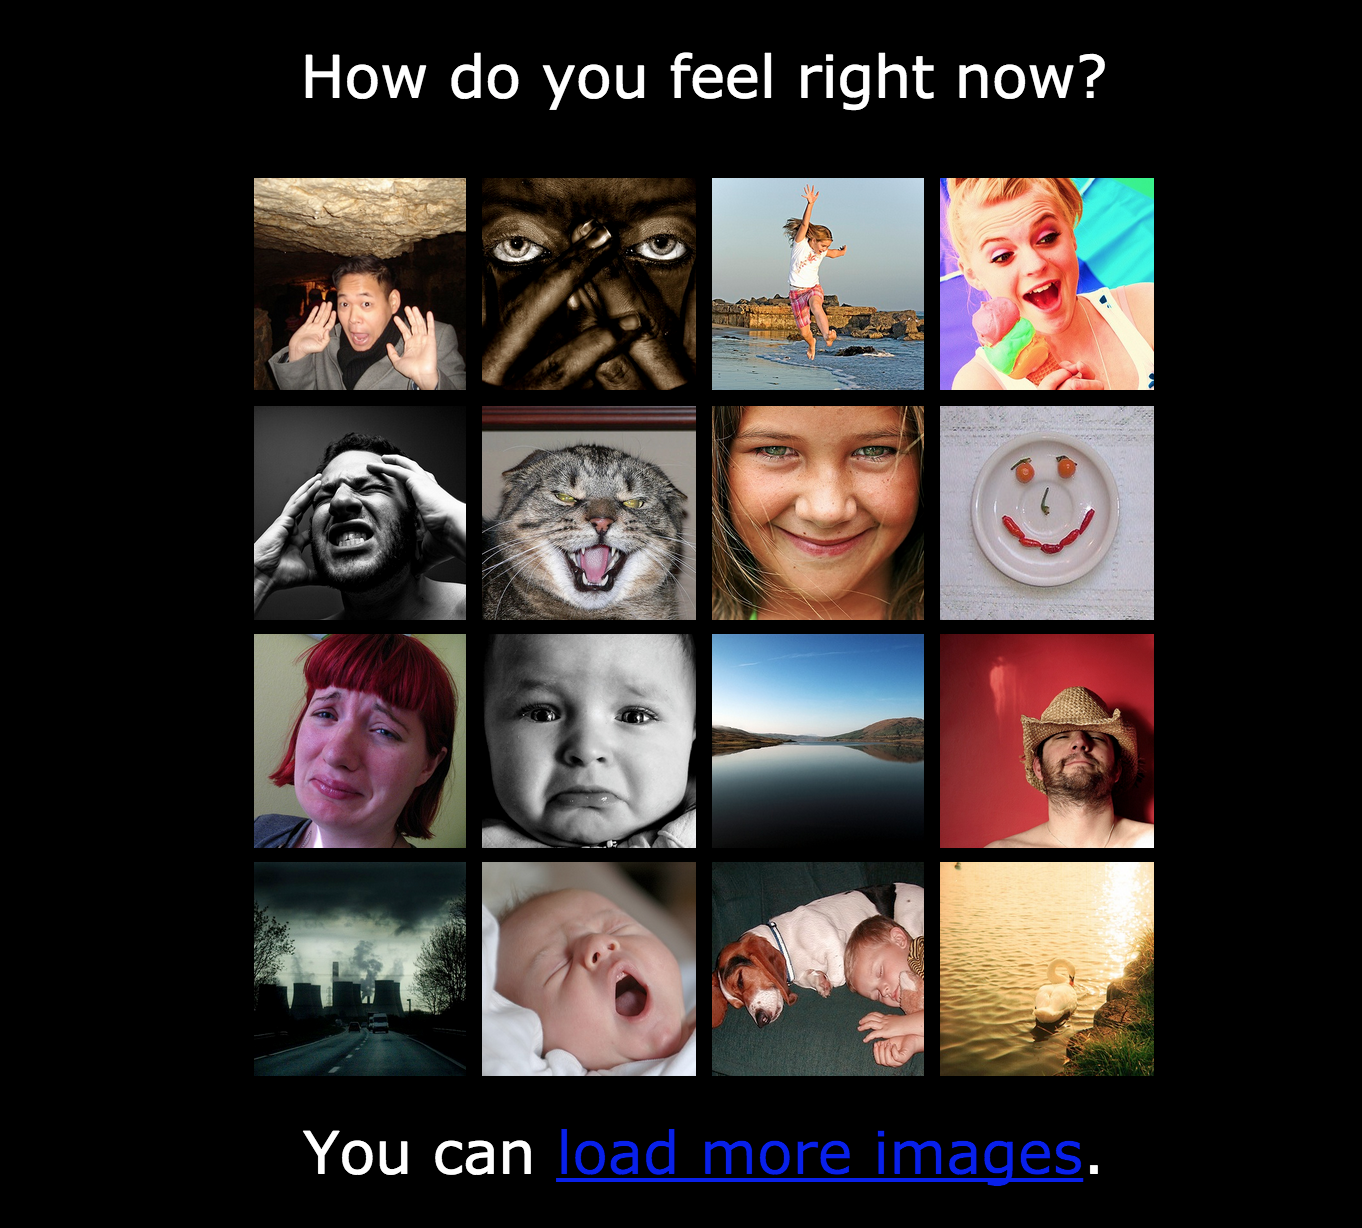
\includegraphics[width=\columnwidth]{pam}
		\label{pam}
		\caption{PAM: the user selects one of 16 grid pictures that reflects their internal emotional state.} 
		\label{pam}
\end{figure} 

\begin{figure}[ht]
	\vskip 0.2in
	\begin{center}
		\centerline{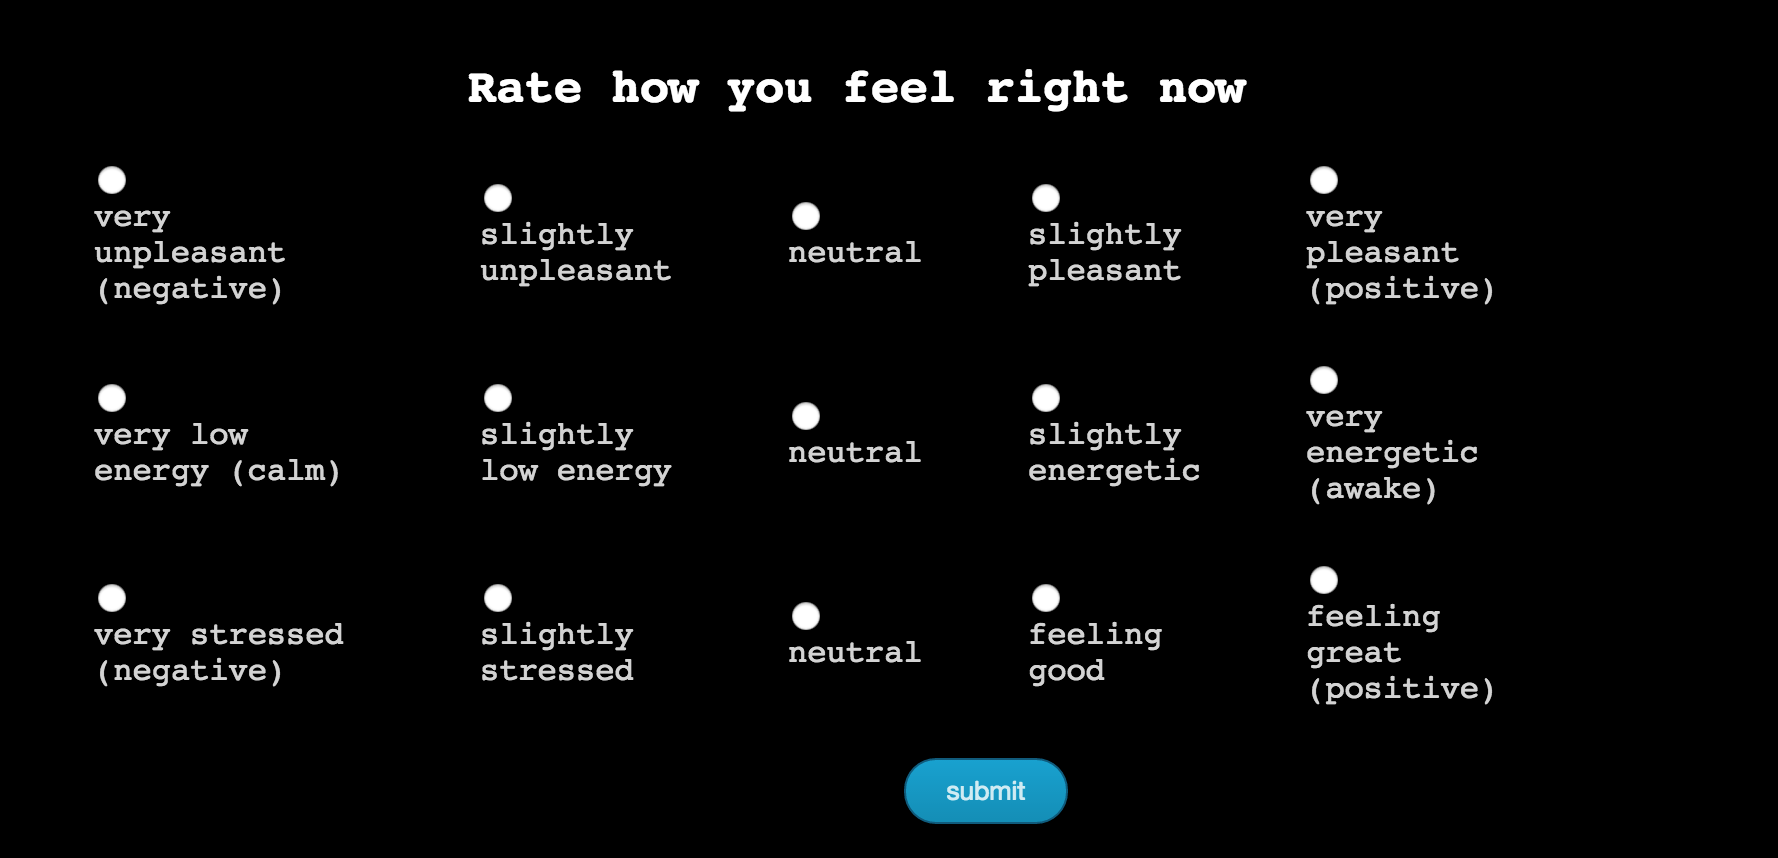
\includegraphics[width=\columnwidth]{ema}}
		\caption{A 3-question survey: the user gets to pick one response out of five categories for each question. 
		}
		\label{ema}
	\end{center}
	\vskip -0.2in
\end{figure} 


\subsection{Data Collection Software}
For visualizing keystrokes heatmap and mouse heatmap, we use WhatPulse \cite{whatpulse}. This can easily be downloaded and installed on the end user system. Since WhatPulse does not provide data to the granularity necessary for conducting our research, a system was built that logs user keystrokes, mouse activities and applications used throughout the day. While there are a few open sourced tools that could have been adopted, a custom application was built because existing tools suffer from poor documentation and/or incomprehensible programming approaches. 

Upon installation, our software tool contains a keystroke logger, a mouse logger, an application logger and a self-report logger. The keyboard and mouse applications continuously logs keystrokes and mouse activities; the foreground application is logged every 3 seconds; while the stress self-report is logged every 30 minutes. The self-report application starts up a PHP server, opens PAM webpage with the user's default browser. Upon selecting a choice from the 16-grid pictures, the response is saved in a file. Thereafter, the 3-question survey is opened as the next webpage, which upon answering a ``thank-you'' page loads. After about 5 seconds, the ``thank-you'' page automatically closes. Self-report application logs user response based on when they responded and not when the page opens. For instance, if the Web page opens at 4pm but the user responds at 7pm, then the response is logged at 7pm. 

Every 15 minutes, a background script checks if all the applications are running or if they have been stopped either manually by the user, another running process, or through a power down of the user computer. This ensures that user logging continues non-intrusively as users do not have to manually start the applications if they were shut down. In order to maintain user access control, every activity application has an icon that appears in the dock so that the user can close the application whenever they want to; users can also delete the data directory if they don't want to partake in the experiment. These intervals for each application were arbitrarily chosen. 

In order to obtain personal visualization of data collected so far, a user has to run the ``view-my-stats'' script. This automatically starts the server and opens up the visualization webpage based using default browser. Due to space limitation, details of this including sample visualization are left out as this feature exists to keep the user informed of their computing habits. 

\subsection{Data Format}
Each activity logged had specific data formats that aided the analysis and visualizations. 

\textbf{mouse logging format:}\\
	time 
	\textpipe \  mouse\textunderscore event  
	\textpipe  \  mouse\textunderscore direction  
	\textpipe \  y=y\textunderscore coordinate \   x=x\textunderscore coordinate\\   
	    \newline
	where mouse\textunderscore event could be \textit{MouseButtonHooker} and
	mouse\textunderscore direction is either of \textit{NSRightMouseUp, NSRightMouseDown, NSLeftMouseUp, NSLeftMouseDown}.
	
For instance: \\
2015-05-03 12:18:55.438360 
MouseMoveHooker 
NSMouseMoved 
y=606.19140625 x=683.0390625

\textbf{keyboard logging format:}\\
time
	\textpipe \  key\textunderscore event  
	\textpipe  \  key\textunderscore direction
	\textpipe \ char=\  char\textunderscore pressed \ 
    key=numeric\textunderscore value
     mods=$['fcn\textunderscore value']$
    is\textunderscore repeat=boolean\textunderscore value.\\
    \newline
    where \  key\textunderscore event is \textit{KeyHooker};  key\textunderscore direction is either of \textit{NSKeyUp, NSKeyDown}; char\textunderscore value is the actual key typed (this shows as \$\$ to protect user privacy), mods is any key command combined with an alphabetic key such as SHIFT, CONTROL, ALTERNATE, etc, which are referred to as fcn\textunderscore value i.e. function value;  is\textunderscore repeat is either of \textit{True, False} depending on if a key is held down or not.\\
    
 For instance: \\
2015-05-03 12:20:28.903225 
        \textpipe \ KeyHooker               
        \textpipe \ NSKeyDown 
        \textpipe \ char=\$\$ 
        mods=$['COMMAND']$
         key=\$\$ 
         is\textunderscore repeat=False
         
\textbf{application logging format:}\\
time \textpipe \  application  \\

For instance:\\
2015-05-07 22:39:09.113787 \textpipe  \  Google Chrome

\textbf{pam logging format:}
time, 
image\textunderscore id: img\textunderscore num, 
cell\textunderscore id: id\textunderscore num, 
pam\textunderscore pa: pa\textunderscore num, 
pam\textunderscore na: na\textunderscore num, 
arousal: arousal\textunderscore num, 
valence: valence\textunderscore num. \\

For instance: \\
time: 2015-04-29 23:47:11, image\textunderscore id: 11, cell\textunderscore id: 4, pam\textunderscore pa: 16, pam\textunderscore na: 3, arousal: 4, valence: 4. \\
where each image has an associated id that identifies the exact picture selected by the user. Details about the scoring mechanism can be found in the PAM literature \cite{pollak2011pam}.

\textbf{ema logging format:}\\
time: 2015-04-27 03:59:49, pleasant\textunderscore state: p\textunderscore state, energy\textunderscore state: e\textunderscore state, stress\textunderscore state: s\textunderscore state. \\
where each of the states are one out of the five options as shown in the 3-point survey question above. 

For instance: \\
time:2015-04-2703:59:49, pleasant\textunderscore state: slightly\textunderscore pleasant, energy\textunderscore state: slightly\textunderscore energetic, stress\textunderscore state: feeling\textunderscore good.

%time: 2015-04-27 03:59:49, pleasant_state: slightly_pleasant, energy_state: slightly_energetic, stress_state: feeling_good

\subsection{Feature Extraction}
We segmented the raw computer usage activities with sliding window size = 1 minute and the extracted three types of computer usage features, \textbf{M}, \textbf{K}, and \textbf{A} for mouse clicks, keystrokes, and application usage within each sliding window. \textbf{M} = $[d_{m}, r_{m}, t_{m}]$, where $d_{m}$ is the total distance of mouse movement, $r_{m}$ is the mouse click rate, and $t_{m}$ is the average mouse button pressed duration. \textbf{K} = $[r_{k_1}, t_{k_1}, r_{k_2}, t_{k_2}, t_{k_i}, ..., r_{k_N}, t_{k_N}]$, i $\in{N}$, where $k_{i}$ stands for different keys and N stands for total number of key types we logged, and $N=9$ in our case, including function keys, letter keys, enter key, tab key, space key, delete key, escape key, arrow key, and all the keys that were pressed (that is, the previous key types were also taken into account), and $t_{k_i}$ is key pressed time for key $k_{i}$.  \textbf{A} = $[t_{a_1}, t_{a_2}, t_{a_j}, ..., t_{a_P}, x]$, j $\in{P}$, where $a_{i}$ stands for different applications, $P$ is the total number of applications users might open when using computers, $t_{a_j}$ is the time users spent on application $a_{j}$, and $x$ is the number of active applications within each time window. To know decide what $P$ is, we first iterated through the users' historical application usage logs.

\subsection{Algorithms}
Since the self-report survey popped up every 30 minutes, we only considered raw computer usage features within the 30-minute duration, if the computer was active,  before the survey is filled out. That is, assuming the user filled out the survey at timestamp $T_end$, and the computer got active at timestamp $T_c$, we only considered raw features with timestamps in $[T_{begin}, T_s)$, where $T_{begin}$=$min(T_{end-1800}, T_c)$. And according to the previous section, we extracted high level features from the raw features among each period and got computer usage samples $S_{T_{begin}}, S_{T_{begin+60}}, ..., S_{T_{end-60}}, S_{T_{end}}$, where each sample $S$ was labeled with the corresponding binary results of users' stress level based on the participants' EMA self-report score. Then we used Decision Tree, Random Forest, support vector machine (SVM), as well as participants' historical data for future stress prediction.

\begin{figure}
	\centering
	\begin{subfigure}
		\centering
		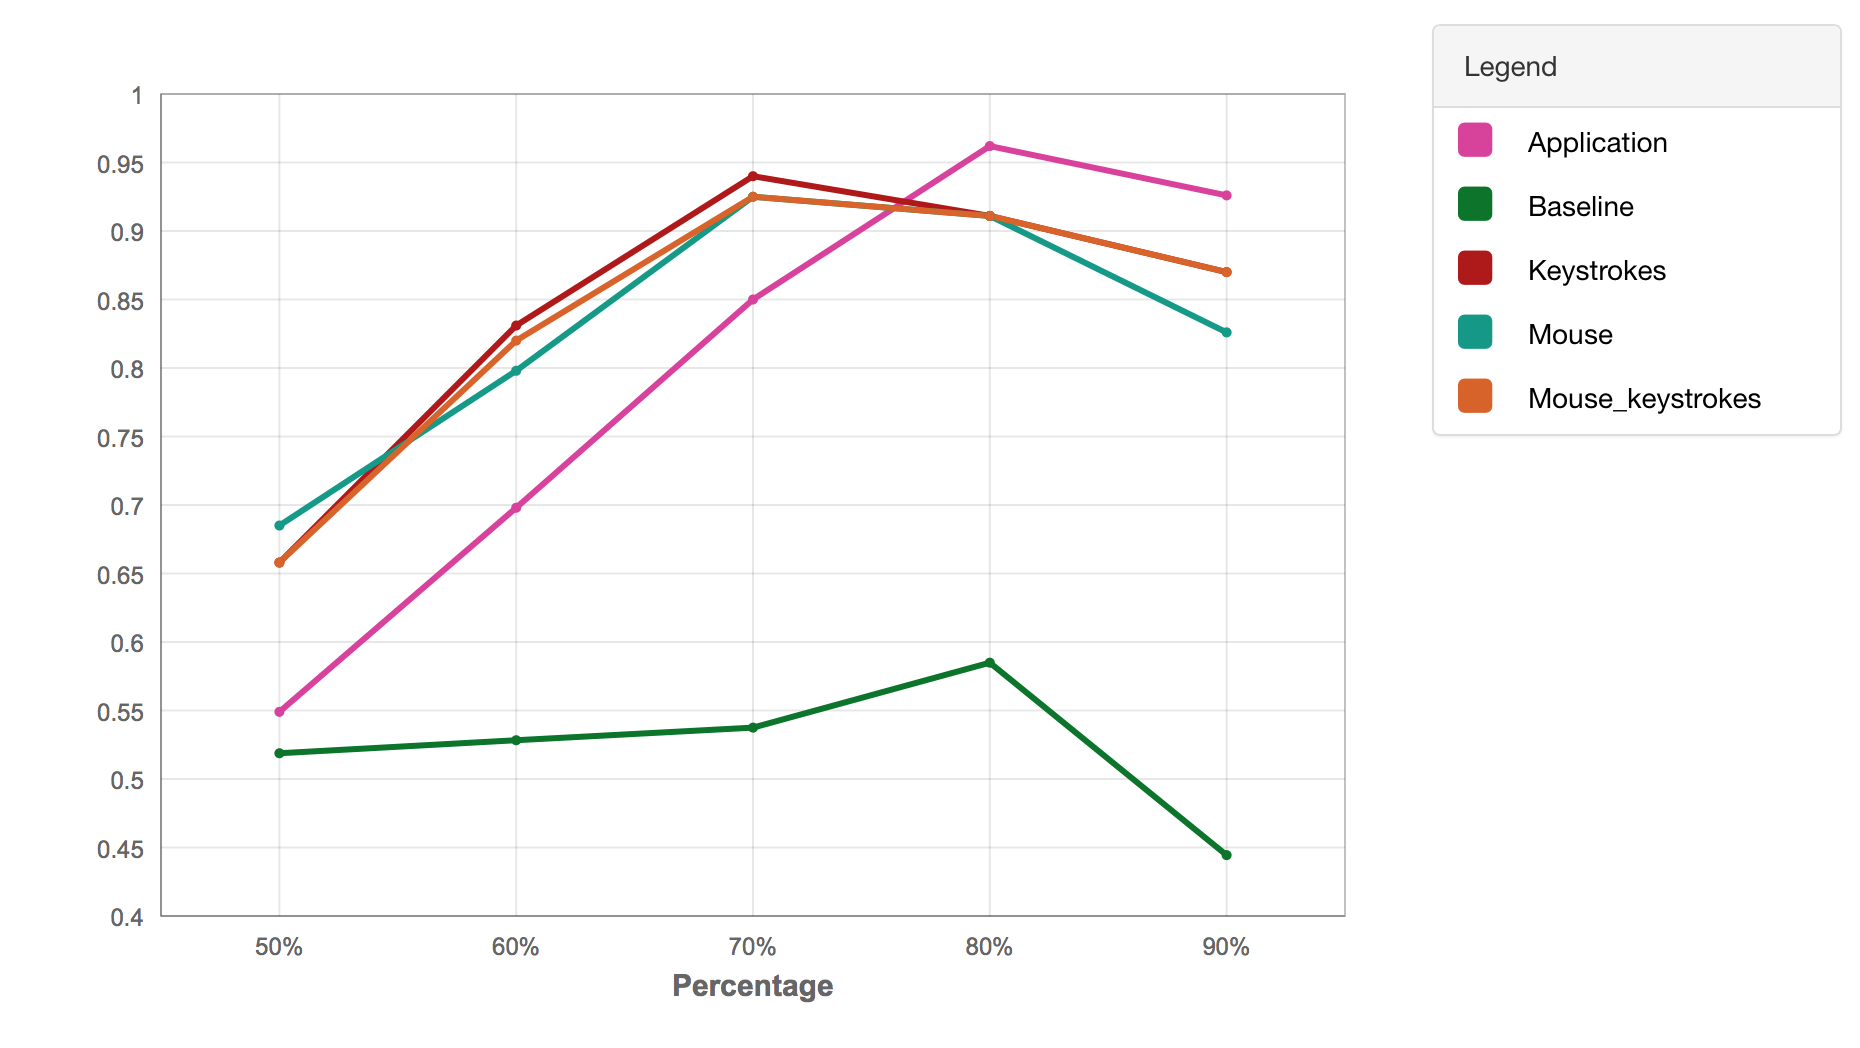
\includegraphics[width=\columnwidth]{DecisionTree.png} {a. Decision Tree}
	\end{subfigure}
	\begin{subfigure}
		\centering
		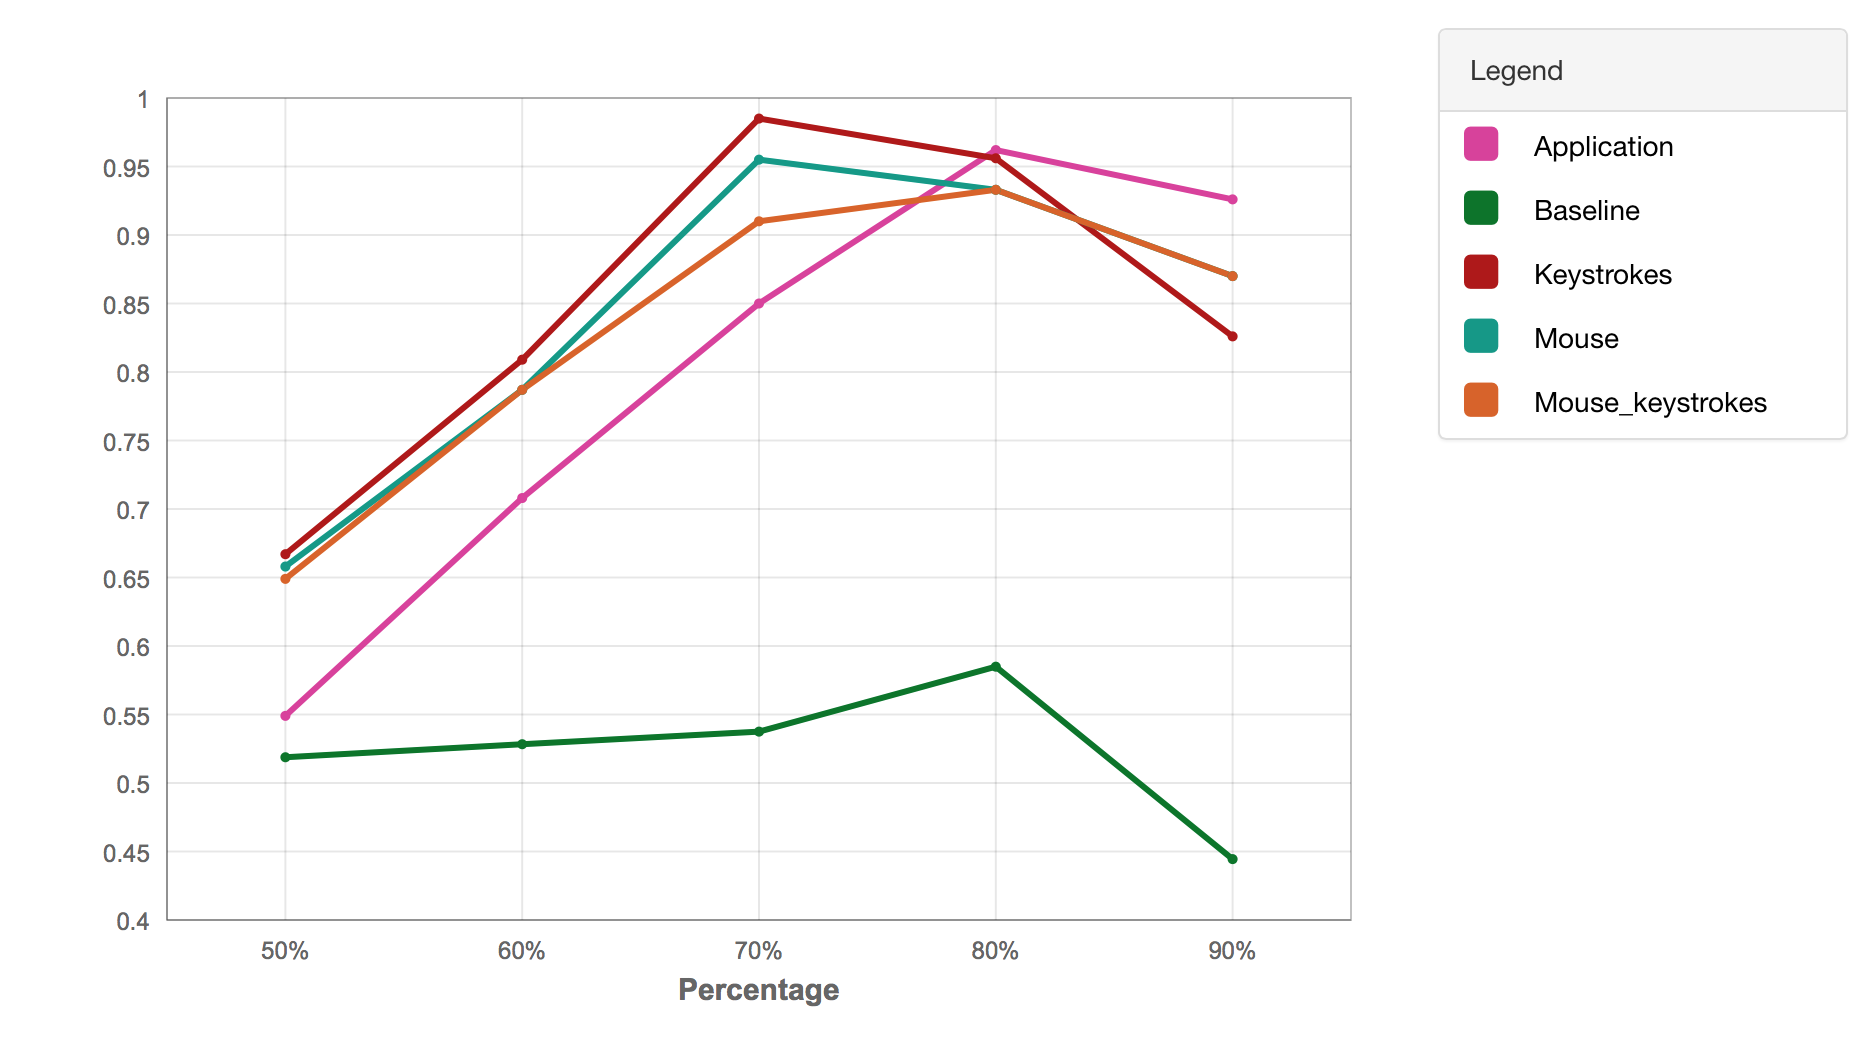
\includegraphics[width=\columnwidth]{RandomForest.png} {b. Random Forest}
	\end{subfigure}
	\begin{subfigure}
		\centering
		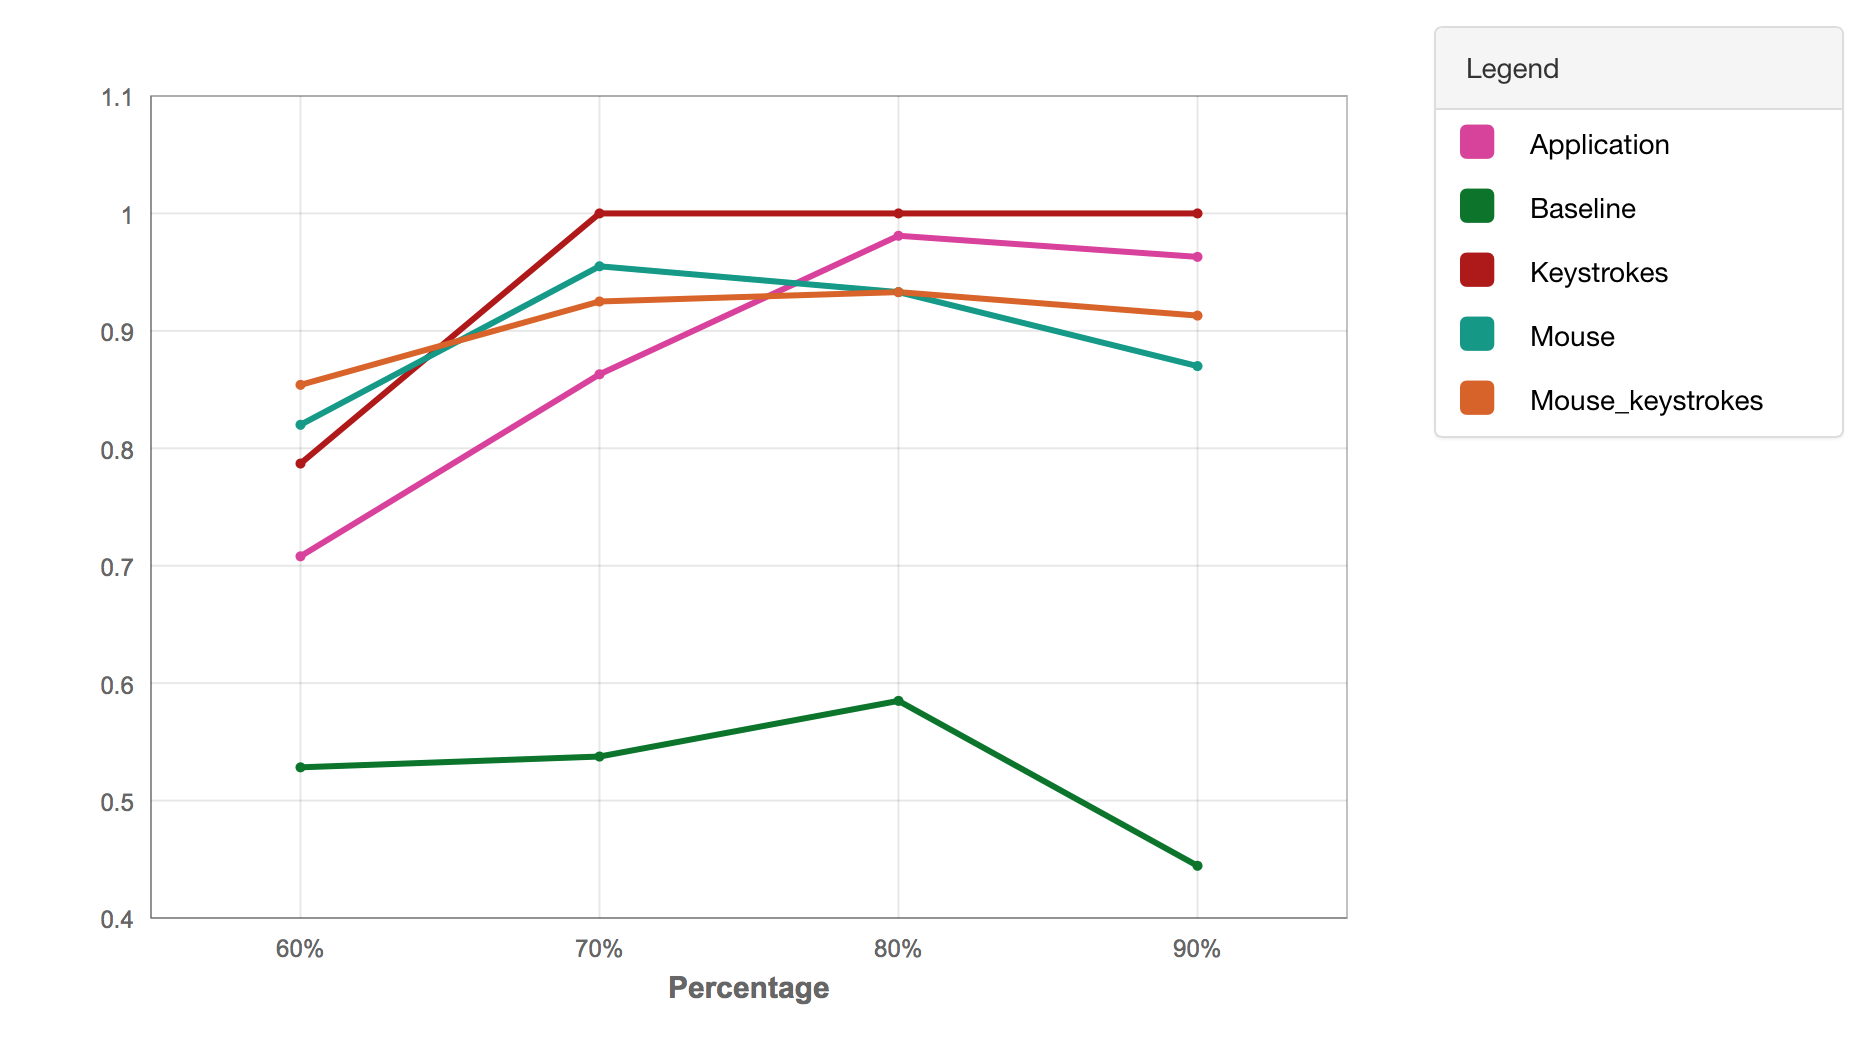
\includegraphics[width=\columnwidth]{SVM.png} {c. SVM}
	\end{subfigure}
	\caption{The accuracy of stress prediction with different algorithms: (a) Decision Tree, (b) Random Forest, (c) Support Vector Machine (SVM) and with different ways of data splits.} \label{prediction}
\end{figure}

\begin{figure}[ht]
	\vskip 0.2in
	\begin{center}
		\centerline{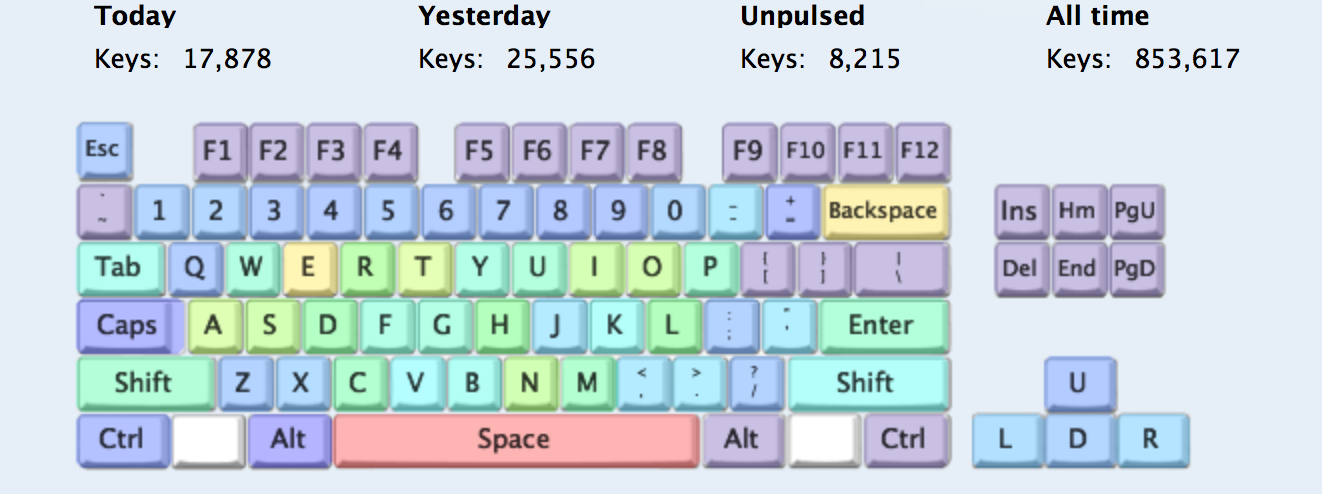
\includegraphics[width=\columnwidth]{keyboard}}
		\label{keyboard}
		\caption{WhatPulse: Keyboard Heatmap}

		\label{icml-historical}
	\end{center}
	\vskip -0.2in
\end{figure} 

\begin{figure}[ht]
	\vskip 0.2in
	\begin{center}
		\centerline{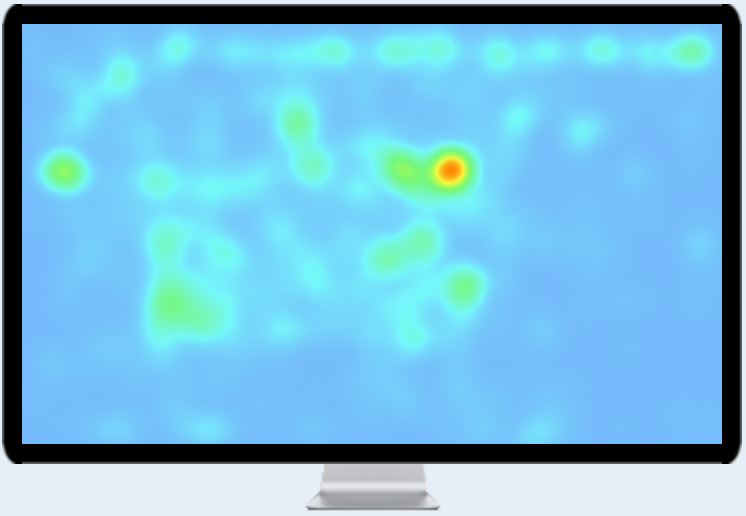
\includegraphics[width=\columnwidth]{mouse_movement}}
		\caption{WhatPulse: Mouse Heatmap
		}
		\label{icml-historical}
	\end{center}
	\vskip -0.2in
\end{figure} 

\section{Results}
Due to time limit and the sensitivity of data initially collected, we could only collect data and train from one participant for consecutive 3 days after the deployment, and we got 352 samples from the deployment. We tried different ways of splits for training and testing, from 50-50 split to 90-10 split,  well as different combinations of features ($M$, $K$, $A$, $M+K$). But we found that the prediction accuracy was very low using only $A$, because during each time window, the participant tended to open just a couple of applications, which made the feature vector of $A$ become very sparse and in turn diminished $A$'s ability for prediction. As a consequence, we decided not to consider all the applications users might use as features. Instead, we only took into account the top 5 frequently used applications as features. That is, the application usage features became $A'=[t_{a_1'}, t_{a_2'}, t_{a_3'}, t_{a_4'}, t_{a_5'}, t_{a_6'}, x]$, where $t_{a_1'}\sim t_{a_5'}$ are the amount of time users spend on the top 5 most frequently used applications during each 1-minute window, and $t_{a_6'}$ is the amount of time users spend on the rest of the applications. After the features were adjusted, the accuracy significantly improved. Figure \ref{prediction} is the accuracy of stress prediction with different algorithms, different combinations of features, as well as different ways of data splits. For the baseline algorithm, it randomly guesses whether the user is stressed or not. The reason why the split for SVM is only down to 60-40 is that the participant's self-report score is quite consistent during the first few days of study, where the participant kept reporting "not-stressed" among the first half of the data we collected. Thus, we would have no training data labeled with "stressed" if we did 50-50 split.

In general, the algorithms achieve the highest accuracy when 70\% $\sim$ 80\% data is used as training data, and the accuracy goes down if more data is used as training data. We have to collect more data and calculate their p-values in order to know what kind of data splits can really achieve the best accuracy and yet the result it obtains is statistical significance, since it is a must for the system to know to how many historical data it has to acquire in order to predict future stress level correctly for the next whole day. 

Initially, we assumed that the more features we used, the better accuracy we would get, but it turned out we got worse accuracy if we built the models using multiple features at the same time, $M+K$ for instance. According to Figure \ref{prediction}, the models trained with $M+K$ performed worse than models trained only with single feature during most of the time. Our speculation is that owning to the limited amount of data, our models tend to over-fit the data if too many features are given. On the other hand, we also noticed that different algorithms perform differently given different types of features. For example, Decision Tree gives the highest prediction accuracy with application usage features, whereas Random Forest somewhat does better with keystrokes features. Therefore, for our next step, we are considering using ensemble methods, combining all these different models together and generating the final prediction with the linear combination of the results given by individual algorithms, where each algorithm is only trained with single type of features with which it is most discriminative.  

\begin{table}[h]
\begin{tabular}{|c|c|c|c|ccc}
\hline
Modalities & \multicolumn{3}{c|}{M}     & \multicolumn{3}{c|}{K}                                                               \\ \hline
Algorithms & DT       & RF      & SVM   & \multicolumn{1}{c|}{DT}    & \multicolumn{1}{c|}{RF}    & \multicolumn{1}{c|}{SVM}   \\ \hline
50\%       & 0.649    & 0.676   & 0.631 & \multicolumn{1}{c|}{0.658} & \multicolumn{1}{c|}{0.631} & \multicolumn{1}{c|}{0.658} \\
60\%       & 0.809    & 0.787   & 0.798 & \multicolumn{1}{c|}{0.843} & \multicolumn{1}{c|}{0.809} & \multicolumn{1}{c|}{0.831} \\
70\%       & 0.821    & 0.896   & 0.94  & \multicolumn{1}{c|}{0.955} & \multicolumn{1}{c|}{0.94}  & \multicolumn{1}{c|}{0.94}  \\
80\%       & 0.911    & 0.911   & 0.956 & \multicolumn{1}{c|}{0.978} & \multicolumn{1}{c|}{0.956} & \multicolumn{1}{c|}{0.911} \\
90\%       & 0.783    & 0.87    & 0.913 & \multicolumn{1}{c|}{0.913} & \multicolumn{1}{c|}{0.826} & \multicolumn{1}{c|}{0.913} \\ \hline
Modalities & \multicolumn{3}{c|}{A}     & \multicolumn{3}{c|}{M+K}                                                             \\ \hline
Algorithms & DT       & RF      & SVM   & \multicolumn{1}{c|}{DT}    & \multicolumn{1}{c|}{RF}    & \multicolumn{1}{c|}{SVM}   \\ \hline
50\%       & 0.703    & 0.703   & 0.703 & \multicolumn{1}{c|}{0.676} & \multicolumn{1}{c|}{0.622} & \multicolumn{1}{c|}{0.667} \\
60\%       & 0.764    & 0.753   & 0.753 & \multicolumn{1}{c|}{0.854} & \multicolumn{1}{c|}{0.775} & \multicolumn{1}{c|}{0.82}  \\
70\%       & 0.97     & 0.955   & 0.94  & \multicolumn{1}{c|}{0.955} & \multicolumn{1}{c|}{1}     & \multicolumn{1}{c|}{0.94}  \\
80\%       & 0.956    & 0.956   & 0.933 & \multicolumn{1}{c|}{0.867} & \multicolumn{1}{c|}{0.911} & \multicolumn{1}{c|}{0.911} \\
90\%       & 0.913    & 0.87    & 0.87  & \multicolumn{1}{c|}{0.957} & \multicolumn{1}{c|}{0.87}  & \multicolumn{1}{c|}{0.826} \\ \hline
Modalities & \multicolumn{3}{c|}{M+A}   & \multicolumn{3}{c|}{K+A}                                                             \\ \hline
Algorithms & DT       & RF      & SVM   & \multicolumn{1}{c|}{DT}    & \multicolumn{1}{c|}{RF}    & \multicolumn{1}{c|}{SVM}   \\ \hline
50\%       & 0.622    & 0.631   & 0.613 & \multicolumn{1}{c|}{0.622} & \multicolumn{1}{c|}{0.649} & \multicolumn{1}{c|}{0.658} \\
60\%       & 0.809    & 0.775   & 0.764 & \multicolumn{1}{c|}{0.787} & \multicolumn{1}{c|}{0.798} & \multicolumn{1}{c|}{0.831} \\
70\%       & 0.925    & 0.91    & 0.955 & \multicolumn{1}{c|}{0.94}  & \multicolumn{1}{c|}{0.94}  & \multicolumn{1}{c|}{0.955} \\
80\%       & 0.889    & 0.911   & 0.933 & \multicolumn{1}{c|}{0.933} & \multicolumn{1}{c|}{0.933} & \multicolumn{1}{c|}{0.933} \\
90\%       & 0.783    & 0.87    & 0.913 & \multicolumn{1}{c|}{0.87}  & \multicolumn{1}{c|}{0.957} & \multicolumn{1}{c|}{0.913} \\ \cline{1-4}
Modalities & \multicolumn{3}{c|}{M+K+A} & \multicolumn{3}{l}{}                                                                 \\ \cline{1-4}
Algorithms & DT       & RF      & SVM   & \multicolumn{1}{l}{}       & \multicolumn{1}{l}{}       & \multicolumn{1}{l}{}       \\ \cline{1-4}
50\%       & 0.613    & 0.64    & 0.631 & \multicolumn{1}{l}{}       & \multicolumn{1}{l}{}       & \multicolumn{1}{l}{}       \\
60\%       & 0.775    & 0.787   & 0.742 & \multicolumn{1}{l}{}       & \multicolumn{1}{l}{}       & \multicolumn{1}{l}{}       \\
70\%       & 0.896    & 0.955   & 0.925 & \multicolumn{1}{l}{}       & \multicolumn{1}{l}{}       & \multicolumn{1}{l}{}       \\
80\%       & 0.889    & 0.956   & 0.956 & \multicolumn{1}{l}{}       & \multicolumn{1}{l}{}       & \multicolumn{1}{l}{}       \\
90\%       & 0.783    & 0.826   & 0.913 & \multicolumn{1}{l}{}       & \multicolumn{1}{l}{}       & \multicolumn{1}{l}{}      
\end{tabular}
\caption{Prediction accuracy with different modalities, algorithms and data splits. $M$ stands for mouse usage, $K$ for keystrokes, and $A$ for application usage.}
\label{results}
\end{table}
 
\subsection{Limitations}
Our dataset is limited. Since recruited participants were PhD students, our prediction model performance cannot be generalized to a broader audience. Since self-report surveys are subject, the definition of stress for different participants will have varying likert scale values. 

Self-report periodically popping up can become annoying to users and/or boring overtime; this invariably means providing misleading training data for our algorithm should users absent-mindedly select a response or none at all. Moreover, emotional states are short-lived and a user can have multiple emotions in a short time so the surveys cannot fully capture the end user's entire emotional states but only a portion.
\begin{table}[h]
\begin{tabular}{|c|c|c|c|ccc}
\hline
Modalities & \multicolumn{3}{c|}{M}     & \multicolumn{3}{c|}{K}                                                               \\ \hline
Algorithms & DT       & RF      & SVM   & \multicolumn{1}{c|}{DT}    & \multicolumn{1}{c|}{RF}    & \multicolumn{1}{c|}{SVM}   \\ \hline
50\%       & 0.649    & 0.676   & 0.631 & \multicolumn{1}{c|}{0.658} & \multicolumn{1}{c|}{0.631} & \multicolumn{1}{c|}{0.658} \\
60\%       & 0.809    & 0.787   & 0.798 & \multicolumn{1}{c|}{0.843} & \multicolumn{1}{c|}{0.809} & \multicolumn{1}{c|}{0.831} \\
70\%       & 0.821    & 0.896   & 0.94  & \multicolumn{1}{c|}{0.955} & \multicolumn{1}{c|}{0.94}  & \multicolumn{1}{c|}{0.94}  \\
80\%       & 0.911    & 0.911   & 0.956 & \multicolumn{1}{c|}{0.978} & \multicolumn{1}{c|}{0.956} & \multicolumn{1}{c|}{0.911} \\
90\%       & 0.783    & 0.87    & 0.913 & \multicolumn{1}{c|}{0.913} & \multicolumn{1}{c|}{0.826} & \multicolumn{1}{c|}{0.913} \\ \hline
Modalities & \multicolumn{3}{c|}{A}     & \multicolumn{3}{c|}{M+K}                                                             \\ \hline
Algorithms & DT       & RF      & SVM   & \multicolumn{1}{c|}{DT}    & \multicolumn{1}{c|}{RF}    & \multicolumn{1}{c|}{SVM}   \\ \hline
50\%       & 0.703    & 0.703   & 0.703 & \multicolumn{1}{c|}{0.676} & \multicolumn{1}{c|}{0.622} & \multicolumn{1}{c|}{0.667} \\
60\%       & 0.764    & 0.753   & 0.753 & \multicolumn{1}{c|}{0.854} & \multicolumn{1}{c|}{0.775} & \multicolumn{1}{c|}{0.82}  \\
70\%       & 0.97     & 0.955   & 0.94  & \multicolumn{1}{c|}{0.955} & \multicolumn{1}{c|}{1}     & \multicolumn{1}{c|}{0.94}  \\
80\%       & 0.956    & 0.956   & 0.933 & \multicolumn{1}{c|}{0.867} & \multicolumn{1}{c|}{0.911} & \multicolumn{1}{c|}{0.911} \\
90\%       & 0.913    & 0.87    & 0.87  & \multicolumn{1}{c|}{0.957} & \multicolumn{1}{c|}{0.87}  & \multicolumn{1}{c|}{0.826} \\ \hline
Modalities & \multicolumn{3}{c|}{M+A}   & \multicolumn{3}{c|}{K+A}                                                             \\ \hline
Algorithms & DT       & RF      & SVM   & \multicolumn{1}{c|}{DT}    & \multicolumn{1}{c|}{RF}    & \multicolumn{1}{c|}{SVM}   \\ \hline
50\%       & 0.622    & 0.631   & 0.613 & \multicolumn{1}{c|}{0.622} & \multicolumn{1}{c|}{0.649} & \multicolumn{1}{c|}{0.658} \\
60\%       & 0.809    & 0.775   & 0.764 & \multicolumn{1}{c|}{0.787} & \multicolumn{1}{c|}{0.798} & \multicolumn{1}{c|}{0.831} \\
70\%       & 0.925    & 0.91    & 0.955 & \multicolumn{1}{c|}{0.94}  & \multicolumn{1}{c|}{0.94}  & \multicolumn{1}{c|}{0.955} \\
80\%       & 0.889    & 0.911   & 0.933 & \multicolumn{1}{c|}{0.933} & \multicolumn{1}{c|}{0.933} & \multicolumn{1}{c|}{0.933} \\
90\%       & 0.783    & 0.87    & 0.913 & \multicolumn{1}{c|}{0.87}  & \multicolumn{1}{c|}{0.957} & \multicolumn{1}{c|}{0.913} \\ \cline{1-4}
Modalities & \multicolumn{3}{c|}{M+K+A} & \multicolumn{3}{l}{}                                                                 \\ \cline{1-4}
Algorithms & DT       & RF      & SVM   & \multicolumn{1}{l}{}       & \multicolumn{1}{l}{}       & \multicolumn{1}{l}{}       \\ \cline{1-4}
50\%       & 0.613    & 0.64    & 0.631 & \multicolumn{1}{l}{}       & \multicolumn{1}{l}{}       & \multicolumn{1}{l}{}       \\
60\%       & 0.775    & 0.787   & 0.742 & \multicolumn{1}{l}{}       & \multicolumn{1}{l}{}       & \multicolumn{1}{l}{}       \\
70\%       & 0.896    & 0.955   & 0.925 & \multicolumn{1}{l}{}       & \multicolumn{1}{l}{}       & \multicolumn{1}{l}{}       \\
80\%       & 0.889    & 0.956   & 0.956 & \multicolumn{1}{l}{}       & \multicolumn{1}{l}{}       & \multicolumn{1}{l}{}       \\
90\%       & 0.783    & 0.826   & 0.913 & \multicolumn{1}{l}{}       & \multicolumn{1}{l}{}       & \multicolumn{1}{l}{}      
\end{tabular}
\caption{Prediction accuracy with different modalities, algorithms and data splits. $M$ stands for mouse usage, $K$ for keystrokes, and $A$ for application usage.}
\label{results}
\end{table}

\section{Future Work}
Future work will involve external sensors for measuring HR, BP, EEG. The current application focuses on batch learning of data already amassed so next iteration will involve online learning especially for making efficient recommendation systems. 

We also plan to use active learning during training and testing in order to overtime reduce the amout of self-reports that occur: in this future approach, the algorithm starts by collecting self-reports periodically. Later, it only prompts the user for self-report after detecting anomalies during data logging.

Further, we intend to collect data for a broader audience and for a longer time to demonstrate more applications of our system and algorithm. 

\section{Conclusion}
In this work, we present a system that predicts user future level of stress based on historical data of keystroke dynamics, mouse activities, application usage, and self report of stress state. Major contributions of our work to existing literature include: building a custom privacy-aware open-sourced stress keylogger, adding computer applications as a contextual feature, deploying diverse machine learning prediction techniques, and providing personalized visualization, which the end user can control. Even though our project is currently limited by the amount of data collected so far, our system and algorithm still demonstrates its functionality; we are confident that our system will demonstrate its full capabilities upon collecting data for a longer period of time. Our work mildly addresses personalized recommendation so future work can building upon more tailored result for each end user. 
% Acknowledgements should only appear in the accepted version. 
\section*{Acknowledgments} 
Special thanks to Prof Daniel Cosley, students of INFO 6010, reviewers of Advanced Machine Learning course (Spring 2015), members of the PAC lab at Cornell University Information Science, and Prof Tanzeem Choudhury, whose guidance was instrumental in this project. 

% In the unusual situation where you want a paper to appear in the
% references without citing it in the main text, use \nocite

\nocite{keystroke}
\bibliography{ml_paper}
\bibliographystyle{icml2012}

\end{document} 


% This document was modified from the file originally made available by
% Pat Langley and Andrea Danyluk for ICML-2K. This version was
% created by Lise Getoor and Tobias Scheffer, it was slightly modified  
% from the 2010 version by Thorsten Joachims & Johannes Fuernkranz, 
% slightly modified from the 2009 version by Kiri Wagstaff and 
% Sam Roweis's 2008 version, which is slightly modified from 
% Prasad Tadepalli's 2007 version which is a lightly 
% changed version of the previous year's version by Andrew Moore, 
% which was in turn edited from those of Kristian Kersting and 
% Codrina Lauth. Alex Smola contributed to the algorithmic style files.  


